71. a) $f(x)=\cfrac{|x^2-x-6|\cdot(x-4)}{3-x}=\cfrac{|x-3|\cdot|x+2|\cdot(x-4)}{3-x}=\begin{cases}-x^2+2x+8,\ x>3,\\ x^2-2x-8,\ x\in[-2;3),\\ -x^2+2x+8,\ x<-2.\end{cases}$
$$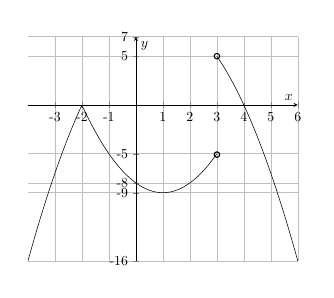
\begin{tikzpicture}[scale=0.5]
\begin{axis}[
    axis lines = middle,
    grid=major,
    legend pos={south west},
    xlabel = {$x$},
    ylabel = {$y$},
    ymin=-16,
    ymax=7,
    xmin=-4,
    xtick={-3,-1,1,3,5,2,-2,4,6},
    xticklabels={-3,-1,1,3,5,2,-2,4,6},
    ytick={ 7, -8, -5,-9,5,-16},
    yticklabels={7, -8,-5,-9,5,-16}           ]
	\addplot[domain=3:6, samples=100, color=black] {(4-x)*(x+2)};
\addplot[domain=-4:3, samples=100, color=black] {abs(x*x-x-6)*(x-4)/(3-x)};
%\addplot[domain=-3:5, samples=100, color=black] {-abs(x-1)};
%\addplot[domain=-3.1:2.5, samples=100, color=red] {70*abs(1-2*abs(abs(x)-2))-10*x^2+10*x-70};
	%\addlegendentry{$\text{Рис. 1}$};
\end{axis}
\draw (4.8,2.7) circle (2pt);
\draw (4.8,5.2) circle (2pt);
\end{tikzpicture}$$
b) Исходя из графика, найдём ответ $p\in(-\infty;-9)\cup(-9;-5)\cup\{0\}\cup[5;+\infty).$\\
